\documentclass[11pt,a4paper]{article}

\usepackage[margin=2.0cm]{geometry}
\usepackage{graphicx}
\usepackage{booktabs}
\usepackage{amsmath,amssymb}
\usepackage{caption}
\usepackage{subcaption}
\usepackage{hyperref}
\usepackage[T1]{fontenc}
\usepackage{times}
\usepackage{microtype}
\usepackage{float}
\usepackage[numbers,sort&compress]{natbib}
\usepackage{parskip}

\setlength{\parskip}{4pt plus 1pt minus 1pt}
\setlength{\parindent}{0pt}

\title{\textbf{COMP534 Assignment~2: 3-Class Lung X-Ray Classification}\\[4pt]
\large Normal / Opacity / Pneumonia}
\author{Ainur Smailova, Nattanan Sottivorakun, Laura Valentina Sierra Peña,  Saif Ur Rehman}
\date{}

\begin{document}
\maketitle
\vspace{-8mm}

% ==================================================================
% (a) EXPERIMENTAL PROTOCOL — 5%
% ==================================================================
\section{Experimental Protocol}

The dataset contains 3{,}475 chest X-ray images ($299\!\times\!299$\,px) across three classes: Normal (1{,}250, 36.0\%), Opacity (1{,}125, 32.4\%), and Pneumonia (1{,}100, 31.7\%), yielding a mild imbalance ratio of 1.14:1. 

\begin{itemize}
    \item \textbf{Data Partitioning}: A \textbf{stratified 80/20 hold-out} split (\texttt{random\_state=42}) creates a training pool (2{,}780) and a locked test set (695), with stratification preserving class proportions to prevent near-zero minority representation in small partitions~\cite{raschka2018}.
    \item \textbf{Validation Strategy}: On the 80\% pool, \textbf{stratified 5-fold cross-validation} ($\sim$2{,}224 train / $\sim$556 val per fold) provides a low-variance generalisation estimate---essential for only 3{,}475 images where a single random split would yield high variance.
    \item \textbf{Evaluation Metric}: Model selection uses \textbf{mean validation macro-F1} across folds rather than accuracy, which misleads under class imbalance by being dominated by the plurality class~\cite{sokolova2009}.
    \item \textbf{Final Evaluation}: The best \emph{configuration} (not weights) is retrained on the full 80\% pool and evaluated \emph{once} on the locked test set, following the strict separation advocated by Hastie et al.~\cite{hastie2009} to prevent optimistic bias from repeated test-set access.
\end{itemize}

All random number generators are seeded at 42 with \texttt{cudnn.deterministic=True} for full reproducibility.
% ==================================================================
% (b) DATALOADER — 12%
% ==================================================================
\section{Data Loading, Preprocessing, and Augmentation}

\subsection{Deterministic Preprocessing (All Splits)}

Each image undergoes the following deterministic pipeline:
\begin{itemize}
    \item \textbf{Resize:} Images are scaled to each model's native resolution ($300 \times 300$ for EfficientNet-B3, $256 \times 256$ for Swin V2, and $224 \times 224$ for MaxViT).
    \item \textbf{CLAHE \cite{rajpurkar2017}:} Applied with \texttt{clip\_limit=2.0} and $8 \times 8$ tiles to enhance local contrast. This process reveals subtle pulmonary opacities often masked by the wide global dynamic range of X-ray imaging, a technique recently validated by EfficientNet achieving a macro-AUC of 0.906 on NIH ChestX-ray14 \cite{sawah2026}.
    \item \textbf{Normalize:} Pixel values are adjusted using ImageNet statistics ($\mu = [0.485, 0.456, 0.406]$, $\sigma = [0.229, 0.224, 0.225]$), which is mandatory for utilizing pretrained weights.
\end{itemize}

\noindent \textbf{Note:} Critically, CLAHE is performed on \texttt{uint8} [0--255] intensities \textit{before} the Normalize step shifts the distribution.

\subsection{Stochastic Augmentation (Training Only)}

Five augmentations model clinically realistic variability (Figure~\ref{fig:aug}):
\begin{itemize}
    \item \textbf{HorizontalFlip}($p\!=\!0.5$) exploits bilateral lung symmetry---a mirrored CXR is clinically indistinguishable from a real one (vertical flip is prohibited as anatomically non-physiological); 
    \item \textbf{Rotate}($\pm10^\circ, p\!=\!0.5$) models patient-positioning variance during acquisition~\cite{castro2020}; 
    \item \textbf{RandomBrightnessContrast}($\pm0.2, p\!=\!0.5$) simulates X-ray exposure variability across machines; 
    \item \textbf{ElasticTransform}($\alpha\!=\!1, \sigma\!=\!50, p\!=\!0.3$) models soft-tissue deformation and breathing-phase variation~\cite{garcea2023}; 
    \item \textbf{GaussNoise}(var$\in$[10,50], $p\!=\!0.3$) simulates quantum noise from low-dose acquisitions.
\end{itemize}

At batch level, \textbf{MixUp}~\cite{zhang2018} ($\alpha\!=\!0.2$) and \textbf{CutMix}~\cite{yun2019} ($\alpha\!=\!1.0$, validated as optimal for medical images~\cite{mediau2025}) alternate randomly ($p\!=\!0.5$). On mixed batches, label smoothing is disabled (MixUp already produces soft labels; combining over-regularises), while unmixed batches use $\varepsilon\!=\!0.1$~\cite{szegedy2016}.

\subsection{Class Imbalance Handling}

\textbf{WeightedRandomSampler} (WRS) assigns each sample weight $w_i = 1/\text{count}(\text{class}_i)$, ensuring approximately equal class representation per batch. Unlike class-weighted loss---which rescales gradient magnitudes but leaves AdamW's moment-estimate covariance dominated by majority-class features---WRS balances gradient covariance in both magnitude \emph{and} sample diversity simultaneously~\cite{buda2018}. WRS is rebuilt per fold from fold-local labels to prevent data leakage. Loss weights are deliberately omitted from \texttt{CrossEntropyLoss} to avoid double-correction.

\begin{figure}[H]
  \centering
  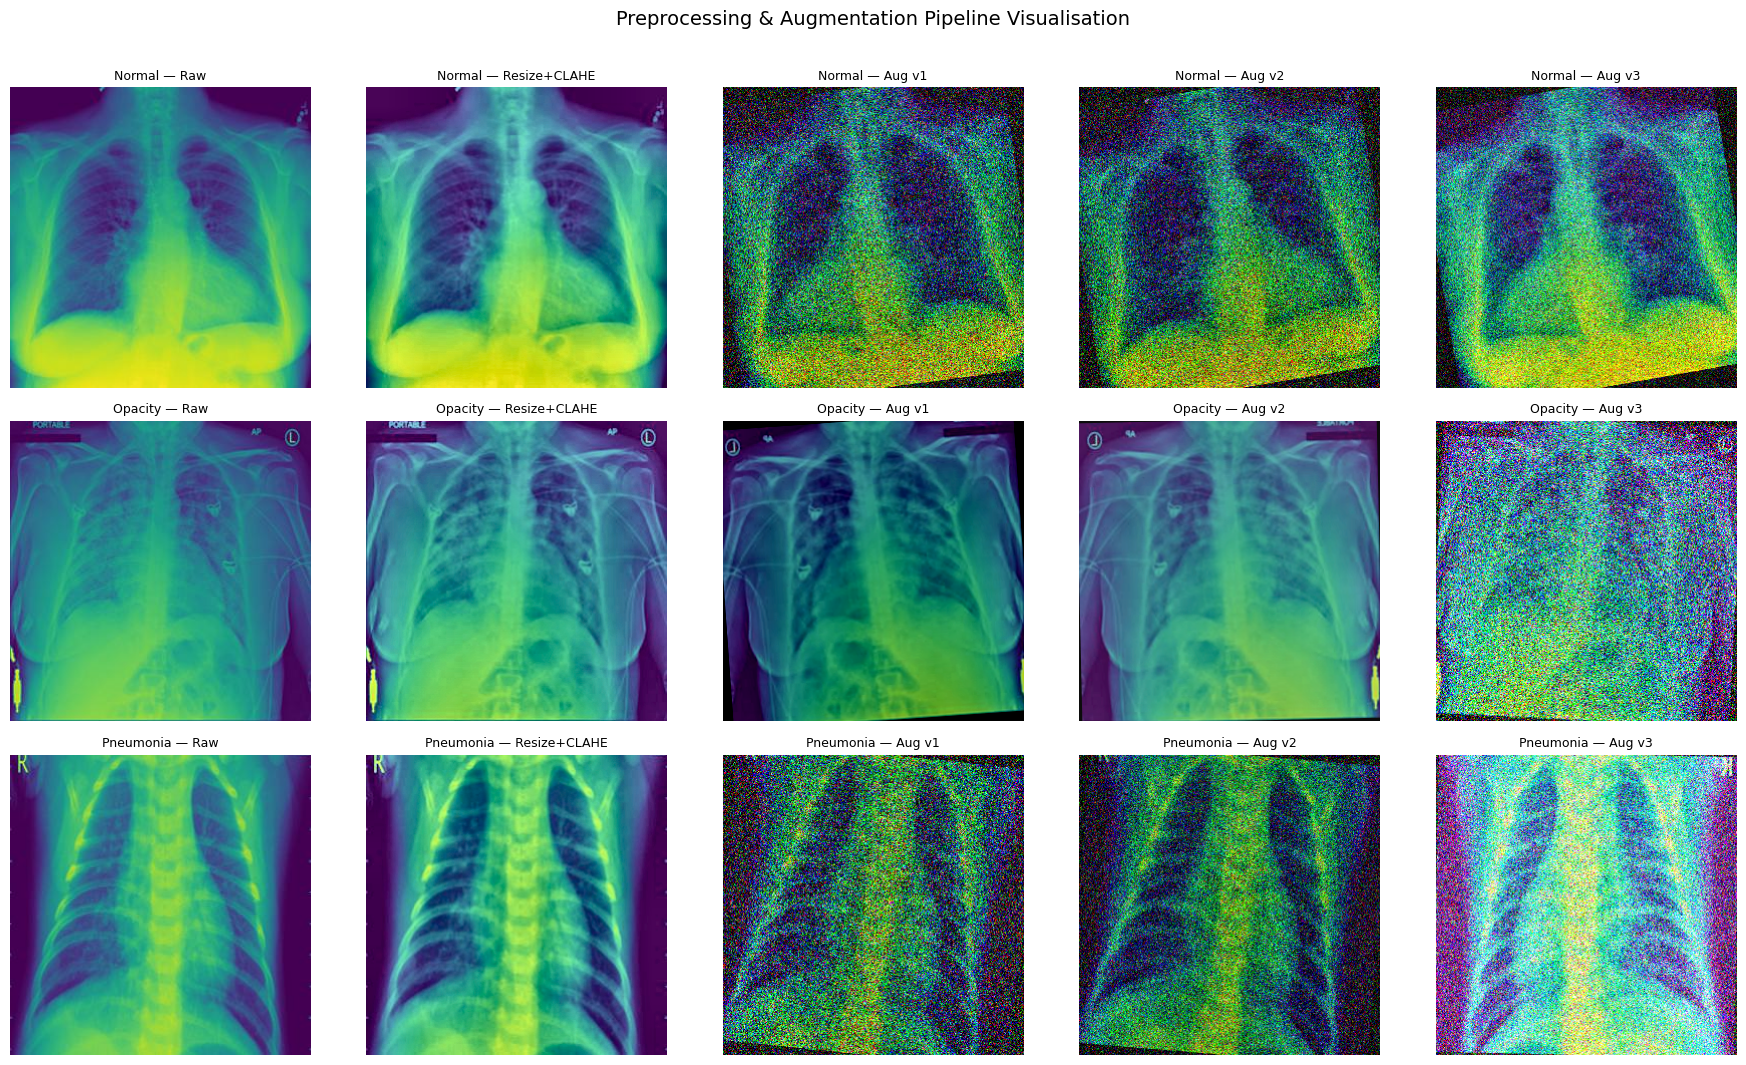
\includegraphics[width=0.92\textwidth]{augmentation.png}
  \caption{Preprocessing pipeline: Raw $\to$ Resize+CLAHE $\to$ stochastic augmentation variants per class.}
  \label{fig:aug}
\end{figure}

% ==================================================================
% (c) NETWORKS, STRATEGIES, COMPONENTS — 13%
% ==================================================================
\section{Network Architectures, Strategies, and Training}

\subsection{Custom CNN: LightXRayCNN ($\sim$0.12M parameters)}

The core design utilizes the following architectural components:
\begin{itemize}
    \item \textbf{Depthwise-separable convolutions}~\cite{howard2017}: A standard $3\!\times\!3$ conv ($C_\text{in}\!\times\!C_\text{out}\!\times\!9$ params) is factored into a depthwise spatial filter ($C_\text{in}\!\times\!9$ params) followed by a $1\!\times\!1$ pointwise channel-mixing filter ($C_\text{in}\!\times\!C_\text{out}$), yielding $\sim$8.9$\times$ parameter reduction.
    \item \textbf{Architecture}: Consists of a stride-2 stem ($3\!\to\!32$ channels) and four DWSep blocks progressively expanding to 256 channels with MaxPool downsampling.
    \item \textbf{Global Average Pooling} (GAP): Replaces fully-connected layers for massive parameter reduction and implicit spatial regularisation~\cite{lin2013}.
    \item \textbf{Classification Head}: Includes Dropout(0.5) + Linear(256,\,3).
    \item \textbf{GELU}~\cite{hendrycks2016}: Replaces ReLU for smoother gradient flow.
\end{itemize}

The design is deliberately parameter-efficient ($\sim$117K parameters), demonstrating that a lightweight architecture can achieve competitive performance (F1=0.8694) when paired with strong preprocessing.

\subsection{Existing Architectures (3 models $\times$ 3 strategies)}

\noindent \textbf{Model Architectures:}
\begin{itemize}
    \item \textbf{EfficientNet-B3}~\cite{tan2019} (10.7M params, 300$\times$300) applies compound scaling---jointly increasing depth, width, and resolution---more principled than scaling one dimension alone.
    \item \textbf{Swin Transformer V2 Small}~\cite{liu2022} (49M params, 256$\times$256) uses shifted-window self-attention with $O(n)$ complexity, producing hierarchical feature maps that capture long-range dependencies critical for distinguishing diffuse opacity from focal pneumonia consolidation.
    \item \textbf{MaxViT Tiny}~\cite{tu2022} (31M params, 224$\times$224) alternates blocked-local and dilated-global multi-axis attention, combining CNN-like locality with transformer-level global context.
\end{itemize}

\noindent \textbf{Training Strategies:}
\begin{itemize}
    \item (1)~\textbf{From scratch} (random init, uniform LR$\!=\!10^{-3}$); 
    \item (2)~\textbf{Feature extraction} (ImageNet backbone fully frozen, only classifier head trains at LR$\!=\!10^{-3}$); 
    \item (3)~\textbf{Fine-tuning} (early layers frozen to preserve low-level features, upper layers trained with differential LR---backbone at $10^{-4}$, head at $10^{-3}$~\cite{howard2018}---preventing catastrophic forgetting while enabling domain adaptation).
\end{itemize}

\subsection{Training Components}

The training pipeline is configured with the following components:
\begin{itemize}
    \item \textbf{Loss}: CrossEntropyLoss with conditional label smoothing ($\varepsilon\!=\!0.1$ on unmixed batches), which softens hard targets to prevent overconfident predictions on a small dataset~\cite{szegedy2016}.
    \item \textbf{Optimiser}: AdamW~\cite{loshchilov2019} (weight decay $10^{-4}$), which correctly decouples L$_2$ regularisation from the adaptive learning rate---unlike vanilla Adam where weight decay is entangled with gradient moments.
    \item \textbf{Gradient clipping} ($\|\nabla\|_\text{max}\!=\!1.0$)~\cite{pascanu2013}: Stabilises fine-tuning where frozen/unfrozen layer boundaries create gradient scale mismatches.
    \item \textbf{Scheduler}: CosineAnnealingLR ($T_\text{max}\!=\!40$, $\eta_\text{min}\!=\!10^{-6}$)---a single cosine descent without restarts, since restarts spike the learning rate and trigger premature early stopping.
    \item \textbf{Early stopping} (patience=10 on val loss): Prevents overfitting on $\sim$2{,}224-image folds while restoring the best checkpoint.
\end{itemize}

% ==================================================================
% (d) RESULTS TABLE — 5%
% ==================================================================
\section{Cross-Validation Results and Model Comparison}

\begin{table}[H]
\centering
\caption{5-fold CV results (mean $\pm$ std macro-F1). Best model selected by highest mean F1.}
\label{tab:cv}
\resizebox{\textwidth}{!}{%
\begin{tabular}{@{}lccl@{}}
\toprule
\textbf{Configuration} & \textbf{Mean Val F1} & \textbf{Std} & \textbf{Per-fold F1} \\
\midrule
LightXRayCNN (scratch) & 0.8694 & 0.0089 & .865\;.866\;.877\;.882\;.857 \\
\midrule
EfficientNet-B3 (scratch) & 0.9026 & 0.0092 & .904\;.903\;.918\;.891\;.897 \\
EfficientNet-B3 (feat.\ ext.) & 0.8856 & 0.0044 & .879\;.891\;.882\;.888\;.889 \\
EfficientNet-B3 (fine-tune) & 0.9379 & 0.0064 & .931\;.940\;.943\;.945\;.929 \\
\midrule
Swin V2-S (scratch) & 0.2924 & 0.0979 & .338\;.176\;.358\;.176\;.413 \\
Swin V2-S (feat.\ ext.) & 0.8895 & 0.0084 & .904\;.892\;.879\;.884\;.890 \\
\textbf{Swin V2-S (fine-tune)} & \textbf{0.9534} & \textbf{0.0106} & \textbf{.945\;.951\;.963\;.968\;.940} \\
\midrule
MaxViT-T (scratch) & 0.6056 & 0.2328 & .651\;.860\;.846\;.350\;.321 \\
MaxViT-T (feat.\ ext.) & 0.8865 & 0.0048 & .896\;.886\;.885\;.884\;.881 \\
MaxViT-T (fine-tune) & 0.9431 & 0.0095 & .938\;.951\;.954\;.945\;.927 \\
\bottomrule
\end{tabular}%
}
\end{table}

\begin{figure}[H]
  \centering
  \begin{subfigure}[b]{0.48\textwidth}
    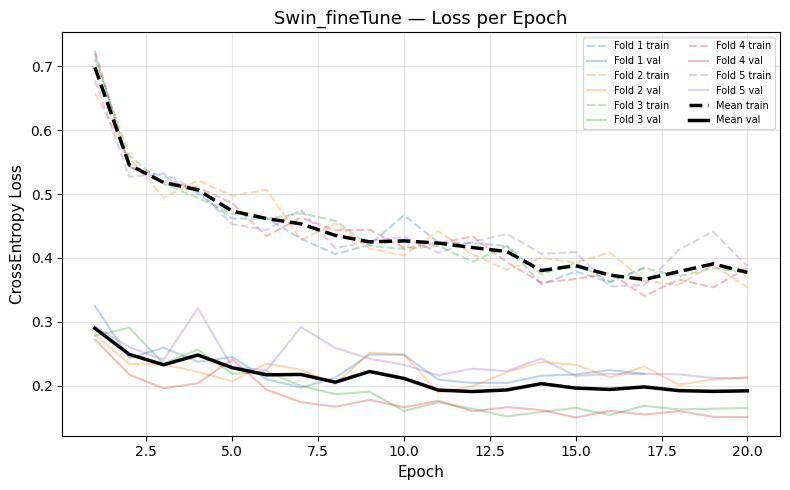
\includegraphics[width=\textwidth]{loss_swin_ft.png}
    \caption{Loss per epoch}
  \end{subfigure}\hfill
  \begin{subfigure}[b]{0.48\textwidth}
    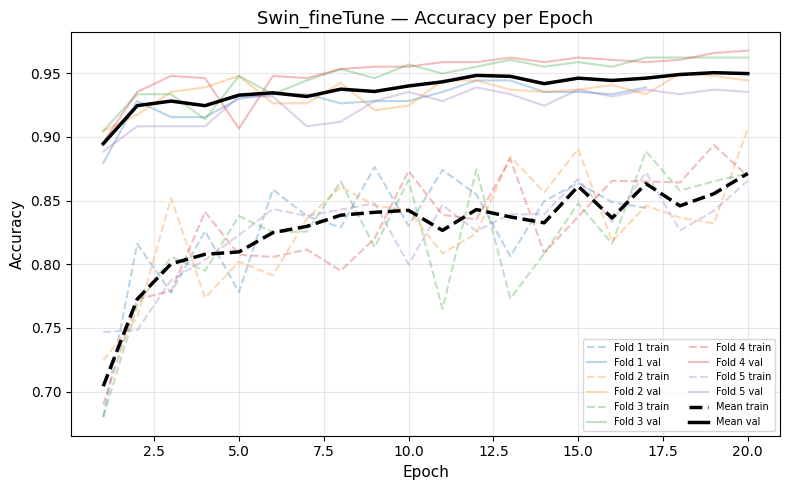
\includegraphics[width=\textwidth]{acc_swin_ft.png}
    \caption{Accuracy per epoch}
  \end{subfigure}
  \caption{Training curves for the best model (Swin V2-S fine-tune) across 5 folds (mean in black).}
  \label{fig:curves}
\end{figure}

Three clear patterns emerge across strategies:
\begin{itemize}
    \item \textbf{Fine-tuning dominates}: all three architectures achieve their best F1 under fine-tuning (Swin: 0.9534, MaxViT: 0.9431, EfficientNet: 0.9379), confirming that differential learning rates effectively adapt pretrained representations to the medical domain. 
    \item \textbf{Scratch training fails for transformers}: Swin (0.2924) and MaxViT (0.6056) collapse without pretrained initialisation---their 49M and 31M parameters vastly exceed what 3{,}475 images can constrain, while EfficientNet's CNN inductive biases (translation equivariance, local receptive fields) enable reasonable scratch performance (0.9026). 
    \item \textbf{Feature extraction provides a stable floor} ($\sim$0.886--0.890) across all architectures with minimal variance, since frozen backbones cannot overfit.
\end{itemize}

The best model, \textbf{Swin V2-S fine-tune}, outperforms all others because shifted-window self-attention captures global spatial dependencies---critical for distinguishing diffuse opacity from focal consolidation---while fine-tuning adapts these representations to the CXR domain. The custom LightXRayCNN achieves 0.8694 with only 0.12M parameters, demonstrating the efficiency of depthwise-separable design.
% ==================================================================
% (e) FINAL EVALUATION — 5%
% ==================================================================
\section{Final Test-Set Evaluation}

The best model was retrained on 90\% of the training pool (10\% internal holdout for early stopping) and evaluated \emph{once} on the locked test set using 5-pass \textbf{TTA}~\cite{shiri2024} (original, H-flip, $\pm5°$ rotation, brightness shift), averaging softmax probabilities before argmax.

We report five metrics, each capturing a genuinely different dimension of performance:

\begin{table}[H]
\centering
\caption{Test-set metrics. Each captures a failure mode the others are blind to.}
\label{tab:test}
\begin{tabular}{@{}llp{5.2cm}@{}}
\toprule
\textbf{Metric} & \textbf{Value} & \textbf{What it uniquely measures} \\
\midrule
Macro-F1 & 0.9479 & Precision-recall balance (hard predictions) \\
Cohen's $\kappa$ & 0.9200 & Agreement above chance (marginal baseline)~\cite{sokolova2009} \\
MCC & 0.9200 & Symmetric confusion-matrix correlation (geometric baseline)~\cite{chicco2020} \\
Log Loss & 0.1888 & \emph{Only} metric on probabilities; penalises overconfident errors logarithmically \\
Balanced Acc & 0.9476 & Pure macro recall; per-class detection equity \\
\bottomrule
\end{tabular}
\end{table}

\begin{table}[H]
\centering
\caption{Per-class precision, recall, and F1 on the test set.}
\label{tab:perclass}
\begin{tabular}{@{}lcccc@{}}
\toprule
\textbf{Class} & \textbf{Prec.} & \textbf{Recall} & \textbf{F1} & \textbf{Support} \\
\midrule
Normal & 0.9209 & 0.9320 & 0.9264 & 250 \\
Opacity & 0.9327 & 0.9244 & 0.9286 & 225 \\
Pneumonia & 0.9909 & 0.9864 & 0.9886 & 220 \\
\midrule
Macro avg & 0.9482 & 0.9476 & 0.9479 & 695 \\
\bottomrule
\end{tabular}
\end{table}

The confusion matrix (Figure~\ref{fig:cm}) reveals that Normal--Opacity confusion dominates errors (15 Normal$\to$Opacity, 17 Opacity$\to$Normal), reflecting their genuine clinical similarity as overlapping radiographic presentations. Critically, only \textbf{3 of 220 Pneumonia cases (1.4\%)} were misclassified as Normal---the highest-severity error, representing a patient requiring treatment being incorrectly discharged. Pneumonia achieves near-perfect F1 (0.9886), indicating the model reliably detects the most clinically urgent pathology. \textbf{HiResCAM}~\cite{draelos2021} (Figure~\ref{fig:gradcam}), chosen over standard GradCAM because Swin's window-partitioned features require element-wise gradient$\times$activation to preserve spatial resolution, confirms that activations concentrate on lung parenchyma: diffuse patterns for Opacity, focal consolidation for Pneumonia, and weak distributed activation for Normal.

\begin{figure}[H]
  \centering
  
\includegraphics[width=0.92\textwidth]{confusion_matrix.png}
  \caption{Confusion matrices: raw counts (left) and row-normalised per-class recall (right).}
  \label{fig:cm}
\end{figure}

\begin{figure}[H]
  \centering
  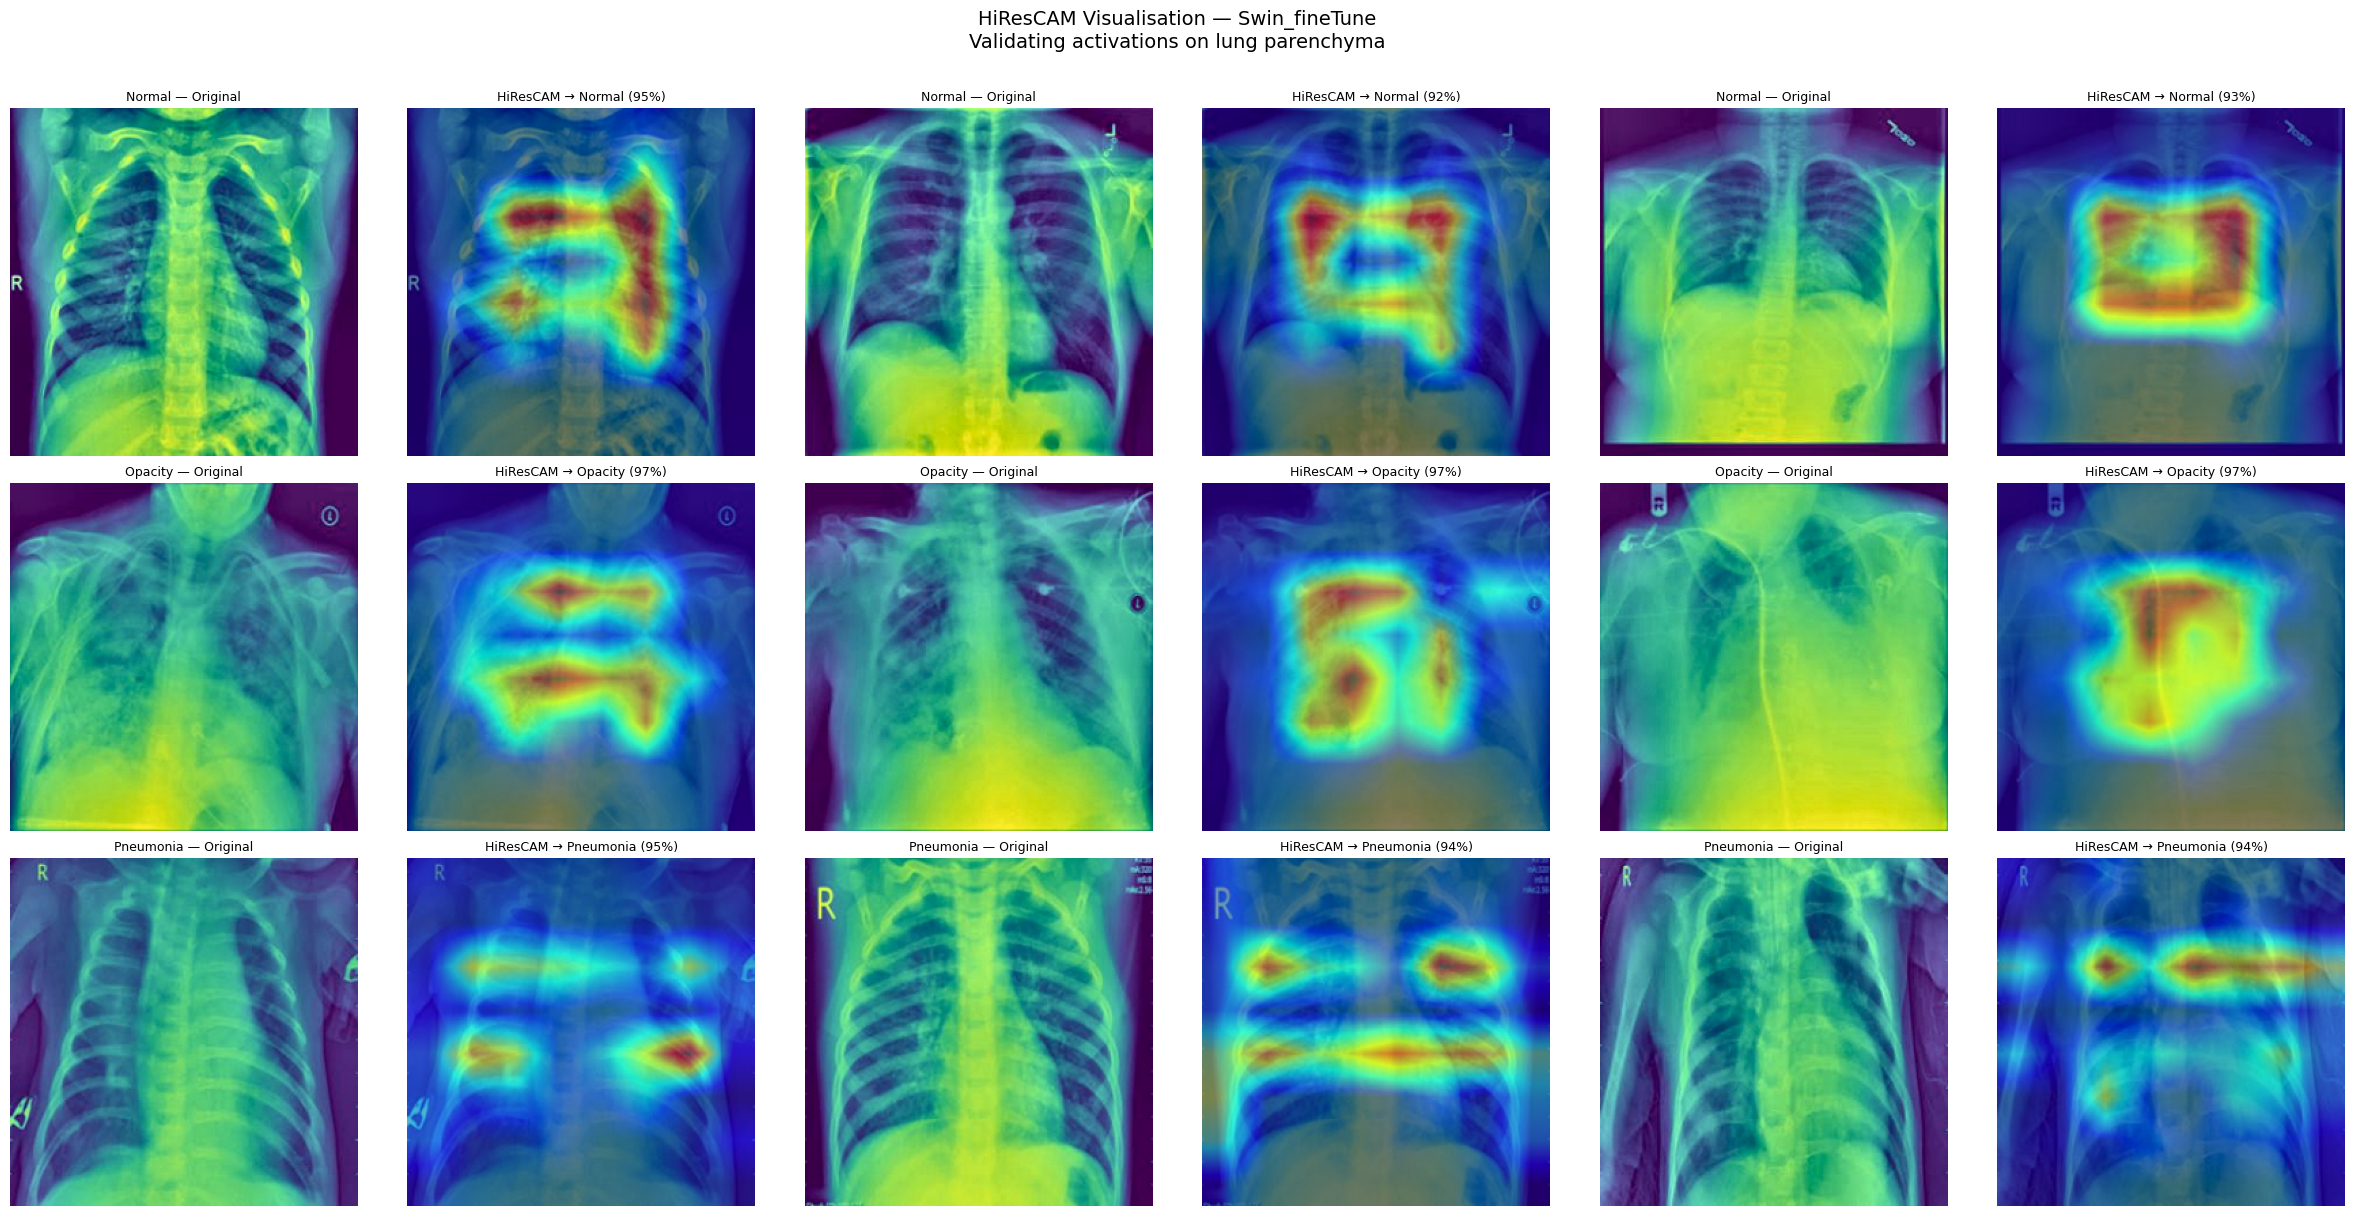
\includegraphics[width=0.92\textwidth]{gradcam.png}
  \caption{HiResCAM heatmaps (Swin V2-S fine-tune). Activations localise to lung fields, validating clinically correct learned representations.}
  \label{fig:gradcam}
\end{figure}

% ==================================================================
\begingroup
\footnotesize
\begin{thebibliography}{24}
\bibitem{raschka2018} S.~Raschka, ``Model evaluation, model selection, and algorithm selection in ML,'' \emph{arXiv:1811.12808}, 2018.
\bibitem{sokolova2009} M.~Sokolova, G.~Lapalme, ``A systematic analysis of performance measures for classification,'' \emph{Inf.\ Process.\ Manag.}, 45(4), 2009.
\bibitem{hastie2009} T.~Hastie \emph{et~al.}, \emph{Elements of Statistical Learning}, 2nd~ed., Springer, 2009.
\bibitem{tan2019} M.~Tan, Q.~Le, ``EfficientNet: Rethinking model scaling for CNNs,'' \emph{NeurIPS}, 2019.
\bibitem{rajpurkar2017} P.~Rajpurkar \emph{et~al.}, ``CheXNet: Radiologist-level pneumonia detection,'' \emph{arXiv:1711.05225}, 2017.
\bibitem{sawah2026} M.~S.~Sawah \emph{et~al.}, ``EfficientNetB0 + CLAHE for CXR classification,'' \emph{Sci.\ Rep.}, 16, 2026.
\bibitem{liu2022} Z.~Liu \emph{et~al.}, ``Swin Transformer V2: Scaling up capacity and resolution,'' \emph{CVPR}, 2022.
\bibitem{tu2022} Z.~Tu \emph{et~al.}, ``MaxViT: Multi-axis vision transformer,'' \emph{ECCV}, 2022.
\bibitem{howard2017} A.~Howard \emph{et~al.}, ``MobileNets: Efficient CNNs for mobile vision,'' \emph{arXiv:1704.04861}, 2017.
\bibitem{hendrycks2016} D.~Hendrycks, K.~Gimpel, ``Gaussian error linear units,'' \emph{arXiv:1606.08415}, 2016.
\bibitem{lin2013} M.~Lin \emph{et~al.}, ``Network in network,'' \emph{arXiv:1312.4400}, 2013.
\bibitem{howard2018} J.~Howard, S.~Ruder, ``Universal language model fine-tuning,'' \emph{ACL}, 2018.
\bibitem{zhang2018} H.~Zhang \emph{et~al.}, ``mixup: Beyond empirical risk minimization,'' \emph{ICLR}, 2018.
\bibitem{yun2019} S.~Yun \emph{et~al.}, ``CutMix: Regularization strategy,'' \emph{ICCV}, 2019.
\bibitem{mediau2025} MediAug, ``Visual augmentation in medical imaging,'' \emph{arXiv:2504.18983}, 2025.
\bibitem{szegedy2016} C.~Szegedy \emph{et~al.}, ``Rethinking the Inception architecture,'' \emph{CVPR}, 2016.
\bibitem{buda2018} M.~Buda \emph{et~al.}, ``Class imbalance in CNNs,'' \emph{Neural Netw.}, 106, 2018.
\bibitem{loshchilov2019} I.~Loshchilov, F.~Hutter, ``Decoupled weight decay regularization,'' \emph{ICLR}, 2019.
\bibitem{pascanu2013} R.~Pascanu \emph{et~al.}, ``On the difficulty of training recurrent neural networks,'' \emph{ICML}, 2013.
\bibitem{garcea2023} F.~Garcea \emph{et~al.}, ``Data augmentation for medical imaging: A systematic review,'' \emph{Comput.\ Biol.\ Med.}, 152, 2023.
\bibitem{castro2020} E.~Castro \emph{et~al.}, ``Causality matters in medical imaging,'' \emph{Nat.\ Commun.}, 11, 2020.
\bibitem{shiri2024} I.~Shiri \emph{et~al.}, ``BayTTA: Uncertainty-aware test-time augmentation,'' \emph{arXiv}, 2024.
\bibitem{chicco2020} D.~Chicco, G.~Jurman, ``Advantages of MCC over F1 score and accuracy,'' \emph{BMC Genomics}, 21, 2020.
\bibitem{draelos2021} R.~Draelos, L.~Carin, ``Use HiResCAM instead of Grad-CAM,'' \emph{arXiv:2011.08891}, 2021.
\end{thebibliography}
\endgroup

\end{document}